\documentclass[12pt]{article}
%\documentclass[12pt]{proc}
\usepackage{graphicx}    % includes epsf
\usepackage{hyperref}
\usepackage{booktabs}
\usepackage{multirow}
\usepackage{siunitx}
\usepackage{threeparttable}
\usepackage{tabularx}
\newcommand{\ra}[1]{\renewcommand{\arraystretch}{#1}}

\begin{document}
%\onecolumn
\title{Beam parameters for the Hall-B RG-M run during November 2021 through January 2022}
\author{}
\date{\today}
\maketitle

Hall-B Run Group M is scheduled to run from November 10, 2021, to January 31, 2022. in experimental Hall B. The CLAS12 is a multipurpose detector system based on a toroidal (forward detector) and a solenoid (central  detector) superconducting magnets. The detector system includes Cherenkov Counters, Drift Chambers, Scintillator Counters, Silicon-strip detectors, Micro-mega gas detectors, and Calorimeters. In this run period CLAS12 will be used in its standard detector and shielding configuration with the Forward tagger off and the Large Moller cone installed. RG-M run will use up to 6 GeV (3 passes) electron beam, with currents up to 300 nA (up to 500 nA on empty target). This run will use several different targets ranging from cryogenic, liquid targets, to heavy solid targets. Targets will be located inside the vacuum scattering chamber that is installed inside the central detector in the center of the 5 T solenoid magnet. 

\begin{table*}
\caption{Target configurations that will be used in RG-M where liquid targets are denoted by "L" and soild targets are listed just as the chemical composition.}\label{tb:target}
\centering
\small
%\ra{1.1}
\begin{threeparttable}
\begin{tabular}{@{}p{1cm}p{2cm}p{2cm}p{1.6cm}p{1.6cm}p{1.6cm}p{1.6cm}p{2cm}@{}}
\toprule
   Energy (GeV)  & Target & Thickness (\si{\centi\metre}) &  Density (\si{\gram\per\centi\metre\cubed}) & Areal Density (\si{\milli\gram\per\centi\metre\squared}) & T/$X_o$\tnote{1} (\%) & Beam Current (\si{\nano\ampere}) & Luminosity\tnote{2}    ($10^{35}$ \si{\per\second\squared \per\centi\metre\squared}) \\
    \midrule
       \addlinespace[0.3cm]
 6.6 & LH     & 5      & 0.071 & 355      & 0.6  & 80 & 1\\ 
 & LD2    & 5      & 0.164 & 820      & 0.7 & 70  & 2\\
 & LHe    & 5      & 0.125 & 625      & 0.7  & 90  & 2\\
 & LAr    & 0.5    & 1.396 & 698     & 3.6  & 80 & 2\\
 &  C \tnote{3}      & 0.2  & 2.20 & 440 & 1.0 & 130 & 2 \\
 &  ${}^{120}$Sn \tnote{3}    & 0.03   & 7.31 & 205 & 2.3 & 277 & 2\\
 &  ${}^{40,48}$Ca    & 0.13    & 1.55 &  200    & 1.2 & 280 & 2 \\
 & Empty  &  --   &  -- & --  & -- & 525 &  -- \\
\addlinespace[0.3cm]
  
  4.4 & LH     & 5      & 0.071 & 355      & 0.6  & 108 & 1.5 \\ 
&   LAr/C    & 0.5/0.2    & 1.396/2.20 & 698/440     & 3.6/1.0  & 110/175  & 3 \\
  & Empty  &  --   &  -- & --  & -- & 450 &  -- \\
  \addlinespace[0.3cm]
  2.2 & LH     & 0.5      & 0.071 & 35.5      & 0.06  & 50 & 0.06 \\ 
 &  LAr/C    & 0.5/0.2    & 1.396/2.20 & 698/440    & 3.6/1.0  &5/8  & 0.13 \\
   & Empty  &  --   &  -- & --  & -- & 380 &  -- \\

\bottomrule
    \end{tabular}
    
     \begin{tablenotes}
     \item[1] Total thickness (T) per radiation length ($X_o$)
     \item[2] per nucleon.
     \item[3] 4-foil target cell.
   \end{tablenotes}
    \end{threeparttable}
 \end{table*}

The target system used for RG-M is the Saclay cryo-target.  This target system has been used in Hall B throughout the 6 GeV and 12 GeV era. RG-M will use the following liquid targets using the Saclay cryo target system (H$_2$, D$_2$, ${}^{4}$He, Ar), and also solid targets (${}^{120}$Sn, C). This target system will be able to support all the targets of interest, except for ${}^{40,48}$Ca which will require encapsulation and will need to be mounted separately. The targets are housed in a vacuum vessel along with the cryogenic system.  A scattering chamber is installed around the target cell area.  This is made from Rohacell foam with a wall thickness of 6.5 mm.  Aluminum windows are used at the entrance and exit of the liquid cells, and at the exit of the scattering chamber.

The details of all components, such as windows and cells, are shown on the beam line drawing, including thicknesses and locations.  The beam line layout is shown in Figures \ref{fig:beamline1} - \ref{fig:beamline4}.


Thwe requirements for beam parameters for RG-M runare summarized in Table~\ref{tab:beam_par}

 \begin{table}[htb]
\caption{Required beam parameters.}\label{tab:beam_par}
\centering
 \begin{tabular}{|c|c|l|}
\hline
Parameter & Requirement &Comments \\ \hline 
Energy (GeV) & 6, 4, 2   & 3, 2, 1 pass  \\  \hline
$\delta$p/p & $\sim 2\times 10^{-4}$ & \\ \hline 
Current (nA) & $\le 300$ &up to 500 nA on empty target  \\  \hline
$\sigma_{xy}$ ($\mu$m) &$ < 200$& As measured by 2H01 harp \\ \hline 
Position stability ($\mu$m) & $< 100$ & On 2H01 and 2H00 ($>30$nA) \\ 
&&BPMs with feedback \\ \hline
Divergence ($\mu rad$) & $< 100$&  \\ \hline 
Beam Halo ($> \pm 5\sigma$) &$< 10^{-5}$&As measured by 2H01 harp \\ \hline
Long term current stability & $< 5$ \% & For $>30$ nA, integrated \\
&&over minutes \\ \hline 
Short term bean intensity & $<10$\%& of the total power, measured \\stability (60 Hz harmonics) && with SLM and halo rates \\ \hline
Bunch charge fluctuations &$< 10$ \% & Measured with DAQ \\ \hline
 \end{tabular}
\end{table}

\begin{figure}[hbt]
\vspace{-2cm}
\begin{center}
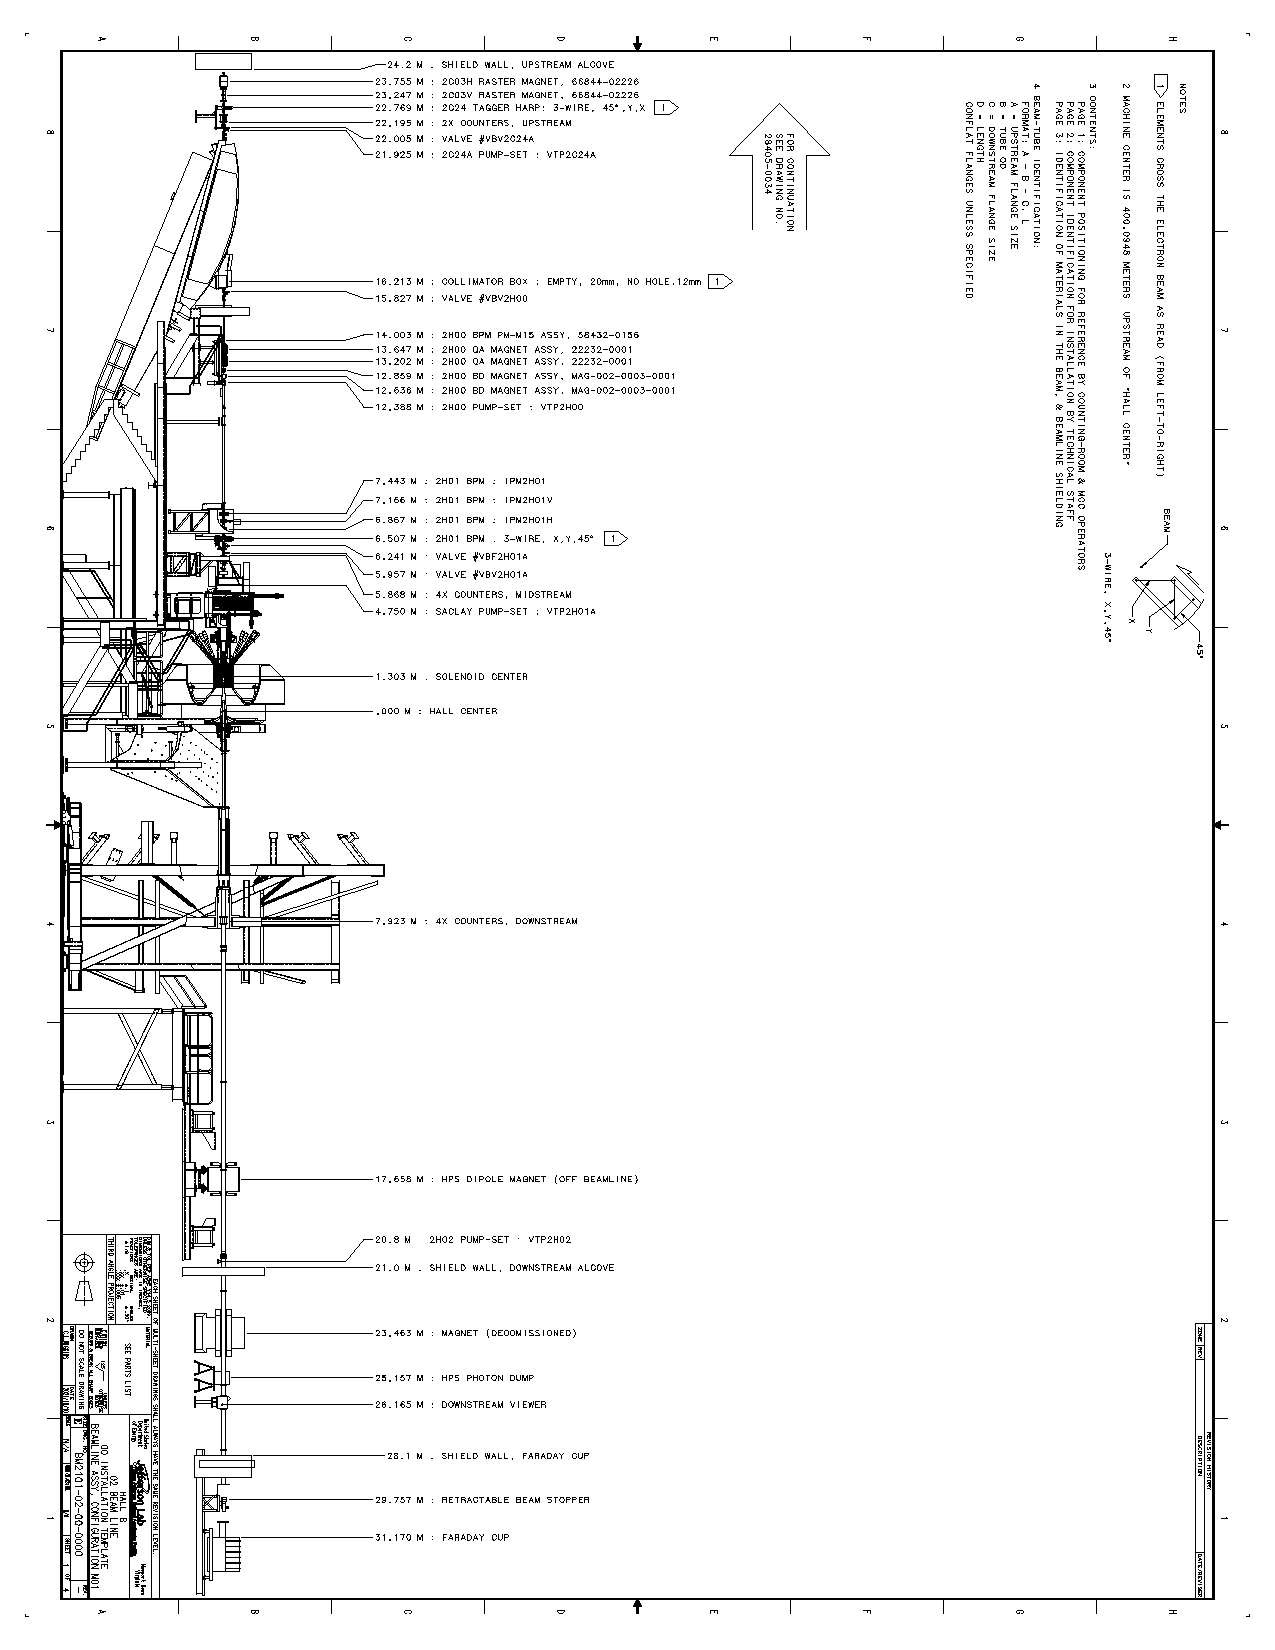
\includegraphics[width=6in]{rgm_beam_page1.pdf}
\caption{ \label{fig:beamline1} The layout of the RG-M beamline. }
\end{center}
\end{figure}

\begin{figure}[hbt]
\vspace{-2cm}
\begin{center}
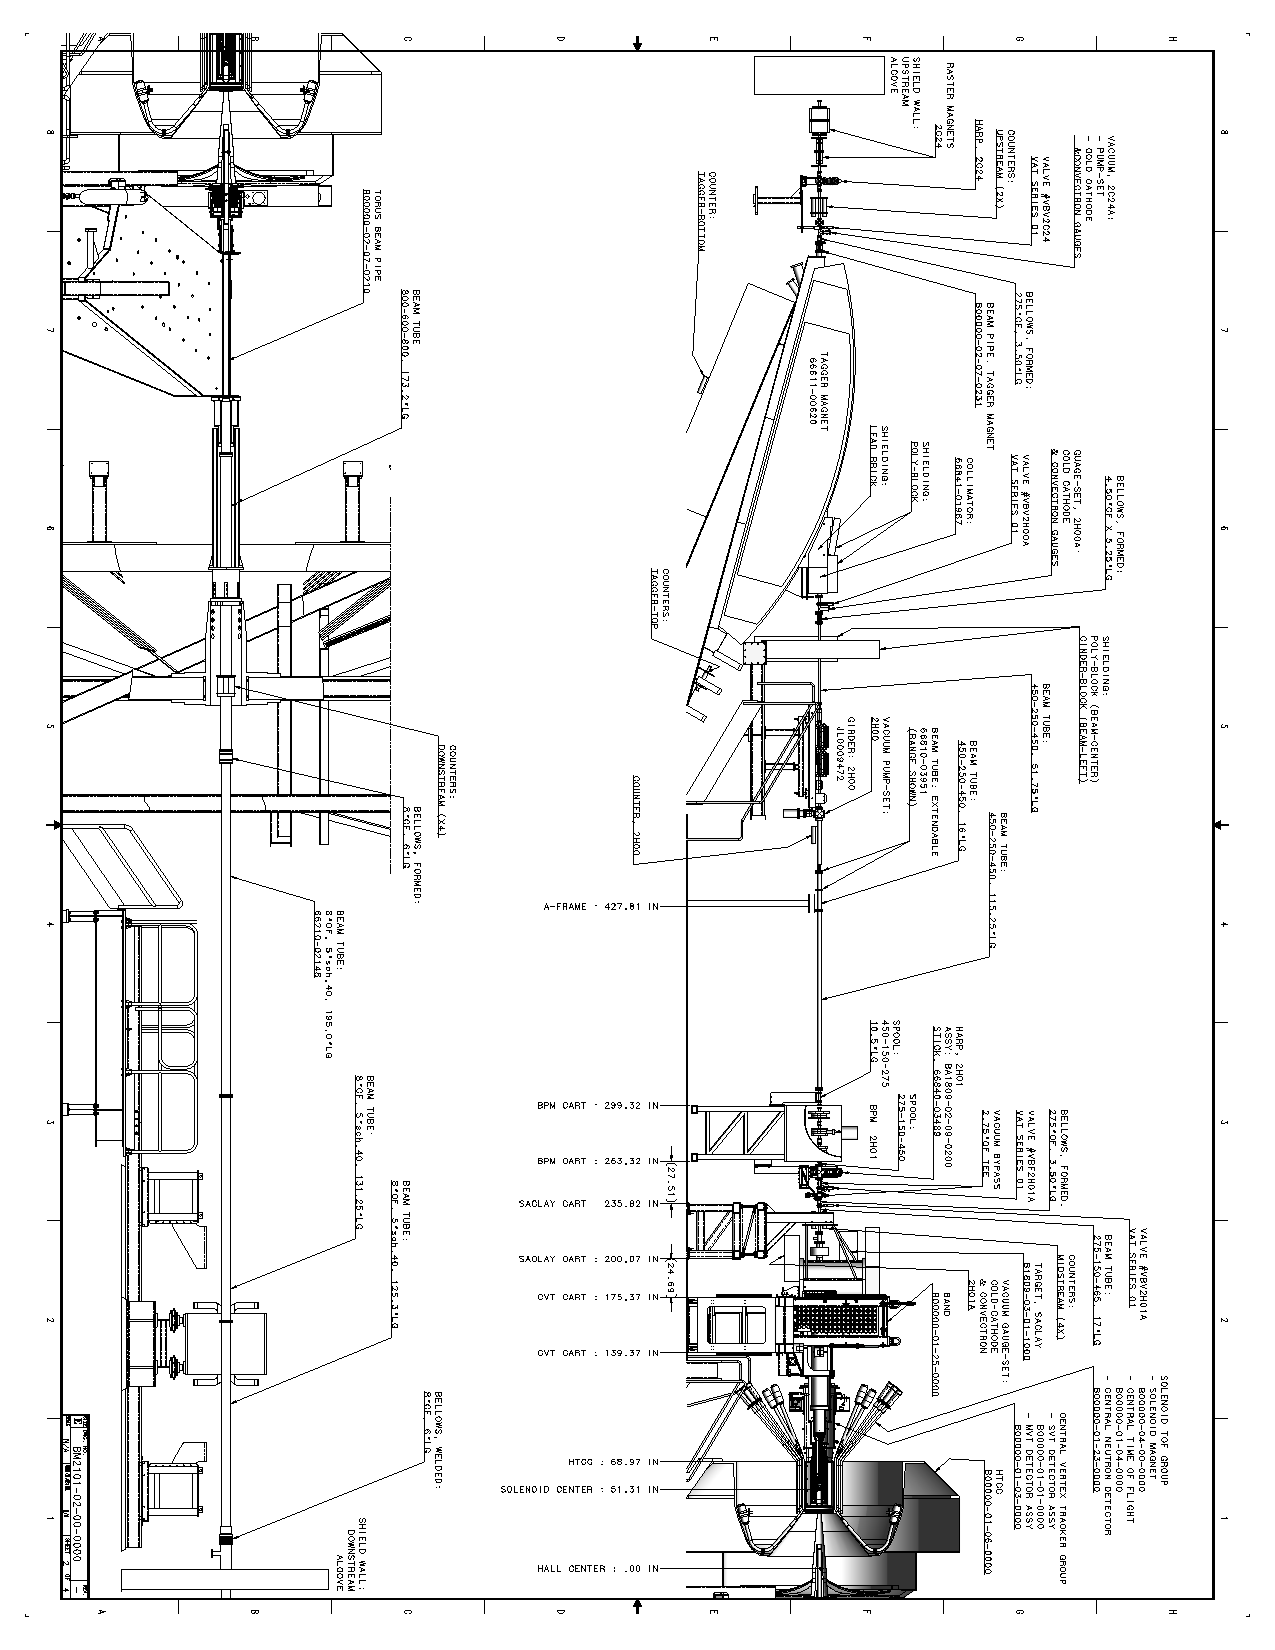
\includegraphics[width=6in]{rgm_beam_page2.pdf}
\end{center}
\caption{ \label{fig:beamline2} 
The layout of the RG-M beamline. }
\end{figure}

\begin{figure}[hbt]
\vspace{-2cm}
\begin{center}
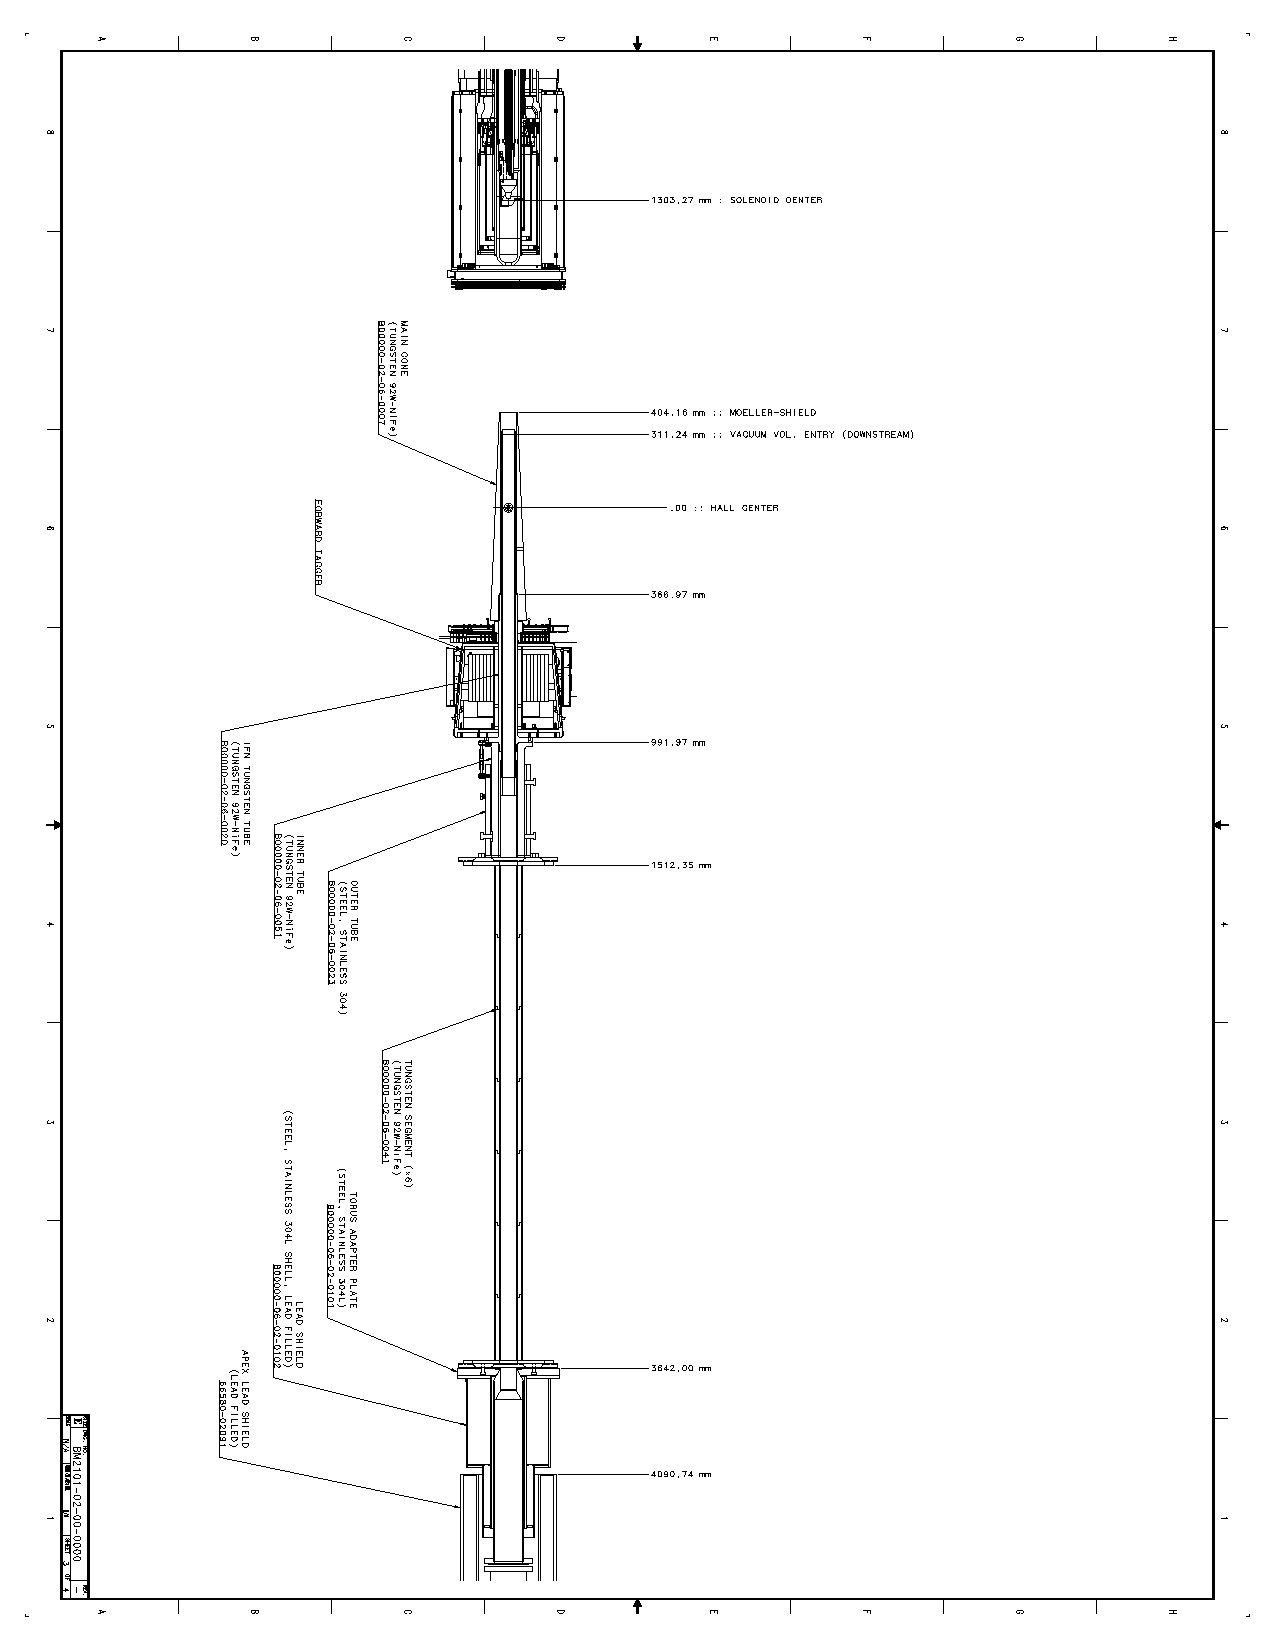
\includegraphics[width=6in]{rgm_beam_page3.pdf}
\end{center}
\caption{ \label{fig:beamline3} 
The layout of the RG-M beamline. }
\end{figure}

\begin{figure}[hbt]
\vspace{-2cm}
\begin{center}
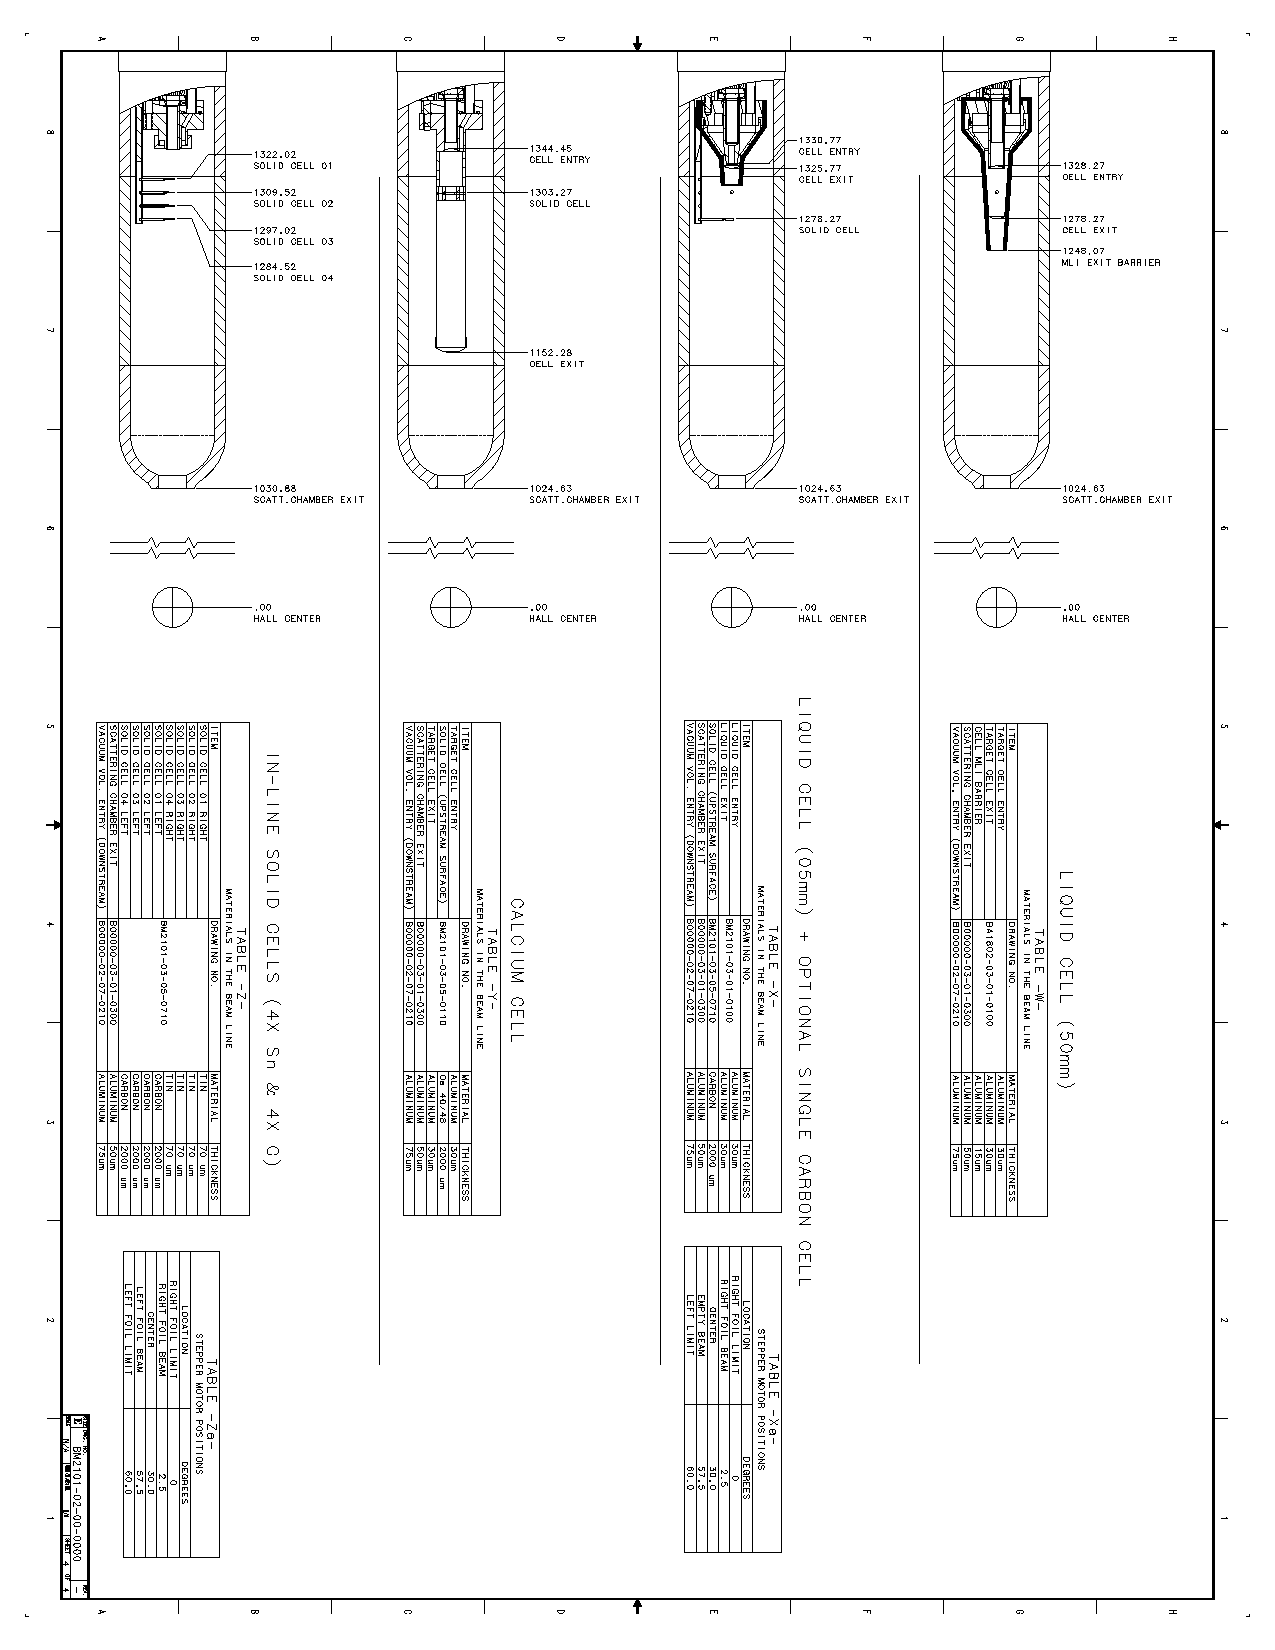
\includegraphics[width=6in]{rgm_beam_page4.pdf}
\end{center}
\caption{ \label{fig:beamline4} 
The layout of the RG-M beamline. }
\end{figure}


For initial beamline tuning and after extended down time (>8 hours) the electron bem will be dumped in the tagger dump. After that the beam will be sent to the Faraday Cup and centered on the target.  For beam currents for which beam power exceeds 175 W on the Faraday Cup (30 nA at 6 GeV, 44 nA at 4 GeV and 87 nA at 2 GeV) the beam blocker will be inserted upstream of the Faraday Cup.

Table~\ref{tab:run_plan} presents the proposed run plan. Depending on the performance of the experiment and accelerator it will be adjusted.


\begin{table*}
\caption{Proposed Run plan}\label{tab:run_plan}
\centering\small
%\ra{1.1}
\begin{tabular}{@{}ccccc@{}}
\toprule
   Energy (GeV)  & Target  & Duration (Hours)  & Target Change Date\\
    \midrule
       \addlinespace[0.3cm]
 6.0 & H    & 48   & November 10, 2021 \\ 
 & Target change H to D & 8 & November 13\\
     & D     & 144   &  November 13    \\
  & Target change D to He & 8 & November 20\\
      & He   & 144  &  November 20\\
  & Target change He to  ${}^{40}$Ca& 22 & November 26\\     
     & ${}^{40}$Ca    & 144  &   November 27  \\
 & Target change  ${}^{40}$Ca to  ${}^{48}$Ca& 12 & December 4\\     
      & ${}^{48}$Ca   & 144  & December 4 \\
  & Target change  ${}^{48}$Ca to C& 12 & December 4\\     
     & C    &  144   &  December 10 \\     
  & Target change  C to Sn & 1 & December 17\\     
     & Sn  &  120  &  December 17 - December 20\\   
    & BREAK  &    &  \\   
    & Sn  & 24  &  January 10 \\   
  & Target change  Sn to Ar & 22 & January  11\\     
     & Ar    & 152    &  January 11\\     
%\addlinespace[0.3cm]

    & Pass change to 1 pass  &    &January 19\\   
    2.1 & Ar     & 40  & January 19\\ 
      & Target change Ar to C & 1 & January 20\\  
      &  C    &  40   & January 18 \\
      & Target change C to D & 22 & January 21\\   
       &  D     &  40   & January 20 \\
      & Target change D to H & 8 & January 23\\   
      &  H    & 8   & January 23 \\
%\addlinespace[0.3cm]

    & Pass change to 2 pass  &    &  January 24\\     
       & Target change H to Ar & 22 & January 24
       \\   4.0 & Ar     & 40    & January 25 \\ 
       & Target change Ar to C & 1 & January 27\\   
     &  C    & 40  & January 27  \\
      & Target change C to H & 8 & January 29\\   
      &  H   & 32  &  January 29\\
%  \addlinespace[0.3cm]


\bottomrule
    \end{tabular}
\end{table*}


\end{document}
